\section{Nội dung đồ án}
\subsection{Sơ đồ UML}
\textit{Sơ đồ UML thể hiện thiết kế hàm, class.}
\begin{figure}[htb]
\centering
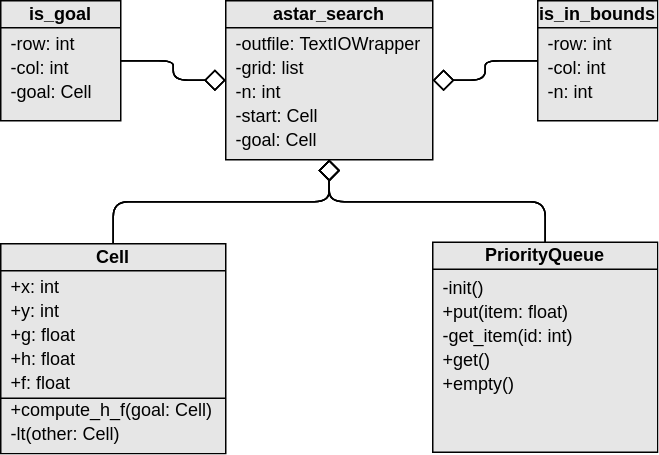
\includegraphics[width=0.98\textwidth]{uml.png} % e.g. insert ./image for image.png in the working directory, adjust scale as necessary
\end{figure}

\subsection{Các hàm chính}
\begin{itemize}
	\item \code{astar-search}
	\begin{itemize}
		\item Tham số đầu vào: \code{outfile} (chứa kết quả), \code{grid} (chứa bản đồ), \code{n} (kích thước bản đồ: n x n), \code{start} - \code{goal} (điểm xuất phát và điểm đích).
		\item Công dụng: Dùng thuật toán A* để tìm đường đi từ một điểm đến một điểm cho trước, trả về \textit{-1} nếu không tìm thấy đường đi.
	\end{itemize}
	
	\item \code{is-in-bounds}
	\begin{itemize}
		\item Tham số đầu vào: \code{row} - \code{col} (tọa độ của ô cần kiểm tra), \code{n} (kích thước bản đồ).
		\item Công dụng: Kiểm tra xem một ô có nằm trong bản đồ hay không.
	\end{itemize}
	
	\item \code{is-goal}
	\begin{itemize}
		\item Tham số đầu vào: \code{row} - \code{col} (tọa độ của ô cần kiểm tra), \code{goal} (ô đích).
		\item Công dụng: Kiểm tra xem một ô có phải là đích hay không.
	\end{itemize}
\end{itemize}

\subsection{Cấu trúc dữ liệu}
\begin{itemize}
	\item Class \code{Cell} với các thuộc tính:
	\begin{itemize}
		\item[+] \code{x}, \code{y}: tọa độ của ô trên bản đồ.
		\item[+] \code{g}: hàm chi phí đi từ điểm bắt đầu đến điểm hiện hành.
		\item[+] \code{h}: hàm heuristic ước lượng khoảng cách từ điểm hiện hành đến đích.
		\item[+] \code{f}: \code{f = g + h}.
	\end{itemize}
	\item \code{PriorityQueue}: hàng đợi ưu tiên.
\end{itemize}

\subsection{Thuật toán chính}
\textit{Thuật toán chính sử dụng là tìm kiếm A*.}
\begin{itemize}
	\item Bước 1: Nếu \code{start} và \code{goal} không nằm trong bản đồ hoặc là vật cản thì kết thúc thuật toán.
	\item Bước 2: Khởi tạo \code{open list}, khởi tạo \code{closed-list} với tất cả giá trị là \code{False}, và khởi tạo \code{parent-list} với tất cả các giá trị có tọa độ \code{(-1, -1)} và \code{f = FLOAT-MAX}. Đưa \code{start} vào \code{open-list}.
	\item Bước 3: Lặp khi \code{open-list} không rỗng:
	\begin{itemize}
		\item Lấy ra node có giá trị \code{f} thấp nhất trong \code{open-list}, gọi là \code{q}. Gán \code{True} cho vị trí của \code{q} trong \code{close list}.
		\item Nếu \code{q} là \code{goal}, tiến hành quay lui thông qua \code{parent-list} để tìm đường đi và kết thúc thuật toán.
		\item Khởi tạo 8 successor xung quanh lân cận 8 của \code{q}.
		\item Với mỗi successor:
		\begin{itemize}
			\item[+] Nếu successor nằm trong bản đồ, không phải là vật cản, và giá trị trong \code{closed-list} là \code{False} thì tiến hành tính \code{g}, \code{h}, \code{f} cho successor này.
			\item[+] Nếu \code{parent} của successor này có \code{f = FLOAT-MAX} hoặc \code{f} lớn hơn \code{f} của successor, ta gán \code{parent} mới cho successor với tọa độ là tọa độ của \code{q}, \code{f} là \code{f} của successor. Và thêm successor này vào \code{open-list}.
		\end{itemize}
	\end{itemize}
	
	\item Bước 4: Nếu \code{open-list} đã rỗng mà chưa tìm thấy đường đi thì kết thúc thuật toán.
	
\end{itemize}
\newpage